\section{Conceitos}

\begin{frame}{Definições}
\begin{block}{Definições}
	\begin{itemize}\itemsep9pt
		\item A atribuição autoral (AA) é uma técnica computacional que visa identificar o autor de um texto a partir de um conjunto de autores possíveis, baseando-se em padrões de estilo deixados pelos autores \cite{Potthast2017}.
		
		\item Do ponto de vista de aprendizado de máquina, a AA pode ser vista como um problema de classificação multi-classes \cite{Stamatatos2009}.
		
		\item A quantificação do estilo de escrita, ou estilometria, compreende um vasto conjunto de medidas e técnicas que buscam extrair uma ``biometria'' textual \cite{Neal2017}.
	\end{itemize}
\end{block}

\begin{block}{}
	Apesar da similaridade com a tradicional tarefa de classificação de documentos, a AA busca elementos inconscientes da escrita que sejam independentes do conteúdo semântico do texto \cite{Keselj2003}.
\end{block}

\end{frame}


\begin{frame}{Conceitos - Fatores que influenciam a AA}

\begin{columns}
	\begin{column}{0.48\textwidth}
		\begin{tcolorbox}[title=Canal,height=2.4cm,valign=center]\selectFont
			$\bullet$ E-mail, jornais, livros, SMS
			
			$\bullet$ Textos mais ou menos formais.                    
		\end{tcolorbox}
	\end{column}
	\begin{column}{0.48\textwidth}
		\begin{tcolorbox}[title=Idioma,height=2.4cm,valign=center]\selectFont
			$\bullet$ Complexidade morfológica e lexical diferentes.
		\end{tcolorbox}
	\end{column}
\end{columns}
\begin{columns}
	\begin{column}{0.48\textwidth}
		\begin{tcolorbox}[title=Tópico,height=2.4cm,valign=center]\selectFont
			$\bullet$ Economia, celebridades, dia-a-dia
			
			$\bullet$ Influencia o vocabulário.                    
		\end{tcolorbox}
	\end{column}
	\begin{column}{0.48\textwidth}
		\begin{tcolorbox}[title=Domínio ou Gênero do texto,height=2.4cm,valign=center]\selectFont
			$\bullet$ Contos, artigos, avaliações de produtos
			
			$\bullet$ Influencia no rigor formal e no vocabulário.
		\end{tcolorbox}
	\end{column}
\end{columns}

\begin{columns}
	\begin{column}{0.48\textwidth}
	\begin{tcolorbox}[title=Tamanho do texto,height=2.4cm,valign=center]
		$\bullet$ Métodos probabilísticos são afetados pelo número de observações.                  
	\end{tcolorbox}
	\end{column}
	\begin{column}{0.48\textwidth}
	\begin{tcolorbox}[title=Número de autores,height=2.4cm,valign=center]
		$\bullet$ O aumento do número de classes requer o aumento do número de classes.                    
	\end{tcolorbox}
	\end{column}
\end{columns}

\end{frame}






%%%%%%%%%%%%%%%%%%%%%%%%%%%%%%%%%%%%%%%%%%%%%%%%%%%%%%%
\begin{frame}{Conceitos - Subtarefas da análise autoral}
	\begin{columns}
		\begin{column}{0.48\textwidth}
			\begin{tcolorbox}[colback=red!5!white,colframe=red!75!black,title=AA de conjunto fechado,height=2.4cm,valign=center]\selectFont
				Os textos do conjunto de teste pertencem a um dos autores candidatos presentes no córpus de treinamento.                    
			\end{tcolorbox}
		\end{column}
		\begin{column}{0.48\textwidth}
			\begin{tcolorbox}[title=AA de conjunto aberto,height=2.4cm,valign=center]\selectFont
				Os textos do conjunto de teste não necessariamente foram escritos por um dos autores do córpus de treinamento                    
			\end{tcolorbox}
		\end{column}
	\end{columns}
	
	\begin{columns}
		\begin{column}{0.48\textwidth}
			\begin{tcolorbox}[title=K-Atribuição ou ordenação ,height=2.4cm,valign=center]\selectFont
				As saídas do classificador são ordenadas pela probabilidade e são retornados os K autores mais prováveis.
			\end{tcolorbox}
		\end{column}
		\begin{column}{0.48\textwidth}
			\begin{tcolorbox}[title=Caracterização,height=2.4cm,valign=center]\selectFont
				São extraídas informações demográficas do autor do texto podem reduzir a lista de candidatos.                    
			\end{tcolorbox}
		\end{column}
	\end{columns}
	
	\begin{columns}
		\begin{column}{0.48\textwidth}
			\begin{tcolorbox}[colback=green!5!white,colframe=green!75!black,title=Verificação,height=2.4cm,valign=center]\selectFont
				Verifica-se se dois documentos foram escritos pelo mesmo autor, não sendo necessário saber quem são os autores.                
			\end{tcolorbox}
		\end{column}
		\begin{column}{0.48\textwidth}
			\begin{tcolorbox}[title=Demais,height=2.4cm,valign=center]\selectFont
				Agrupamento, Ligação e Quebra de estilo.                    
			\end{tcolorbox}
		\end{column}
	\end{columns}

\end{frame}


%%%%%%%%%%%%%%%%%%%%%%%%%%%%%%%%%%%%%%%%%%%%%%%%%%%%%%%
\begin{frame}{Conceitos - Tipos de conhecimentos usados}

A abordagem estilométrica tradicional utiliza as seguintes fontes de conhecimento:

\begin{itemize}
	\item {\bf Categoria lexical:} tamanho médio das palavras, número de letras maiúsculas, quantidade de dígitos, tamanho das sentenças, etc.
	
	\item {\bf Categoria sintática:} frequência da pontuação, palavras de função, frases começando com maiúscula, etc.
	
	\item {\bf Categoria semântica:} contagem das palavras, analisadores semânticos, {\it word embeddings}, etc.
	
	\item {\bf Categoria estrutura:} indentação, tamanho do parágrafo, etc.
	
	\item {\bf Categoria específica de domínio:} palavras-chave, {\it tags} HTML, {\it emoticons}, nomes de produtos.
\end{itemize}
\end{frame}


%%%%%%%%%%%%%%%%%%%%%%%%%%%%%%%%%%%%%%%%%%%%%%%%%%%%%%%
\begin{frame}{Conceitos - Tipos de conhecimentos usados}

Outra classificação possível e simplificada dos conhecimentos utilizados na AA pode ser a utilização das famílias baseadas em palavras e caracteres.


\begin{tcolorbox}[colback=blue!1!white,colframe=blue!35!black,title=Palavras,valign=center]
	\begin{itemize}
		\item As palavras mais frequentes são independentes de domínio e utilizadas de forma inconsciente \cite{Kestemont2014}.
		\item {\bf Palavras de função} (do inglês, {\it function words}) compreende artigos, preposições, locuções adverbiais, e outros.\\
		\item Capturam semântica e elementos de conexão entre sentenças.
		\item Diversas ferramentas são preparadas para usar a unidade {\it palavra}.
	\end{itemize}			
\end{tcolorbox}

\end{frame}

%%%%%%%%%%%%%%%%%%%%%%%%%%%%%%%%%%%%%%%%%%%%%%%%%%%%%%%
\begin{frame}{Conceitos - Tipos de conhecimentos usados}\selectFont

	\begin{tcolorbox}[colback=green!1!white,colframe=green!35!black,title=Caracteres,valign=center]
		\begin{itemize}
			\item As sequências de caracteres são considerados os modelos mais efetivos para AA \cite{KjellWF94,Neal2017}.
			\item Os {\bf caracteres mais frequentes (CNG)} (do inglês, {\it common n-grams}) \cite{Keselj2003,Sapkota2014}.
			\item São independentes de idioma.
			\item Não precisam de {\it stemming} pois lidam bem com idiomas flexionais.
			\item Geram vetores de contagem mais densos que os vetores de palavras.
			\item Os n-gramas de caracteres conseguem capturar pontuação, utilização de espaços, preferências temporais, palavras de função de tamanho curto.
			\item O trabalho em \citeonline{aa-Sapkota2015} mostra que apesar de independente de idioma nem todos os {\it char n-gramas} tem a mesma origem.
		\end{itemize}

	\end{tcolorbox}
\end{frame}

%%%%%%%%%%%%%%%%%%%%%%%%%%%%%%%%%%%%%%%%%%%%%%%%%%%%%%%
\begin{frame}{Conceitos - Modelos computacionais}
\begin{tcolorbox}[title=Modelo tradicional de representação textual - BOW,valign=center]\selectFont
	\begin{itemize}
		\item Hipótese distribucional aplicada a documentos \cite{Turney2010}
		\item Modelo de n-gramas
		\item Conhecimentos: Caracteres, Palavras, POS
		\item TF-IDF
		\item TF-IDF equações alternativas utilizadas nos experimentos:
			\begin{itemize}\selectFont
				\item $ TF_{sublinear} = 1 + \log TF_{t,d}$  $\longrightarrow$ Definição I do SMART. 
				\item $
				IDF_{Suavizado}(t,D) = log\left (
				\frac{D}{DF(t)}
				\right ) + 1
				$
			\end{itemize}
	\end{itemize}	
\end{tcolorbox}
\end{frame}


\begin{frame}{Conceitos - Modelos computacionais}
\selectFont
\begin{columns}
	\begin{column}{0.60\textwidth}
		\begin{tcolorbox}[title=Modelo de representação distribuída,height=7cm,valign=center]\selectFont
			\begin{itemize}
				\item Hipótese distribucional aplicada símbolos
				\item Modelos neurais de língua natural \cite{Bengio2003}
				\item Aprendizado não supervisionado
				\item Transferência de conhecimento
				\item {\it Word embeddings} 
				\begin{itemize}\selectFont
					\item Representa cada palavra, ou símbolo, em k dimensões, sendo k menor que o tamanho do vocabulário.
					\item Word2Vec \cite{Mikolov2013}
					\item Doc2Vec \cite{QuocLe2014}
					\item FastText \cite{bojanowski2017enriching}
				\end{itemize}
			\end{itemize}
		\end{tcolorbox}		
	\end{column}
	\begin{column}{0.40\textwidth}
		\begin{tcolorbox}[title=Modelo Word2Vec,height=7cm,valign=center]\selectFont
			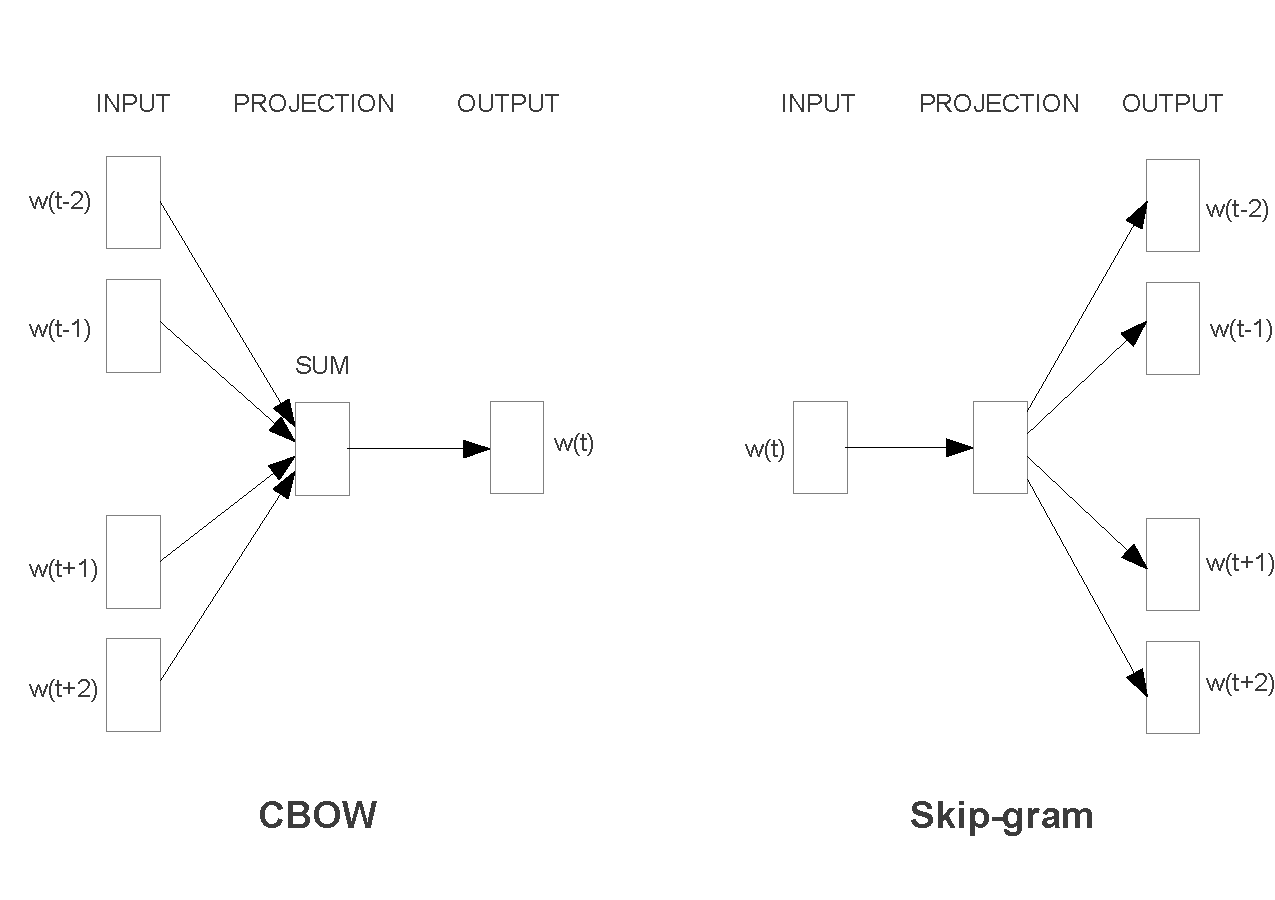
\includegraphics[trim=350 20 0 20,clip,width=.95\textwidth]{images/efficient-models.pdf}
			Fonte: \citeonline{Mikolov2013}
		\end{tcolorbox}		
	\end{column}
\end{columns}
\end{frame}




\begin{frame}{Modelos computacionais baseados em distância}
\selectFont
	As medidas, ou funções, de distância devem obedecer quatro propriedades \cite{deza2009encyclopedia}:
	\begin{enumerate}\selectFont
		\item $D(A,B) >= 0 $ para todo $A$ e $B$, D é positiva.
		\item $D(A,B) = 0 $ se e, somente se, $A = B$.
		\item $D(A,B) = D(B,A) $, $D$ é uma função simétrica.
		\item $D(A, C) <= D(A, B) + D(B, C)$, a desigualdade triangular.
	\end{enumerate}


	\begin{columns}
	\begin{column}{0.48\textwidth}
		\begin{tcolorbox}[colback=red!5!white,colframe=red!75!black,title=Distância de cosseno,height=2cm,valign=center]\selectFont
			$
			Cossenos \left ( A,B \right ) = 1 -\frac{A\cdot B}{\left \| A \right \| \left \| B \right \|}
			$            
		\end{tcolorbox}
	\end{column}
	\begin{column}{0.48\textwidth}\selectFont
		\begin{tcolorbox}[title=Manhattan,height=2cm,valign=center]\selectFont
			$
			Manhattan \left ( A,B \right )= \sum_i {\left| A_i - B_i \right|}
			 $     
	\end{tcolorbox}
	\end{column}
	\end{columns}


	\begin{columns}
		\begin{column}{0.48\textwidth}
			\begin{tcolorbox}[colback=blue!5!white,colframe=blue!75!black,title=Jaccard,height=2cm,valign=center]\selectFont
			$
			Jaccard(A,B) = \frac{\left | A \cap B \right |}{\left | A \cup B \right |}
			$
			
			Interseção binária
			\end{tcolorbox}
		\end{column}
		\begin{column}{0.48\textwidth}\selectFont
			\begin{tcolorbox}[title={MinMax, ou Jaccard generalizado},height=2cm,valign=center]\selectFont
				$
				MinMax (A,B) = \frac{ \sum_{i}^{n}{ min(A_i,B_i|}}{\sum_{i}^{n}{max(A_i,B_i)}}
				$      
			\end{tcolorbox}
		\end{column}
	\end{columns}

\end{frame}


\begin{frame}{Modelos computacionais baseados em distância}
\selectFont
\begin{tcolorbox}[colback=blue!5!white,colframe=blue!75!black,valign=center,title=Regra $\Delta$ de Burrows ]\selectFont
	\begin{equation}
	\begin{aligned}
	\Delta Burrow \left ( A, B \right) = \frac{1}{N}\sum_{i=1}^{N}\left | Zscore(A_i,C_i) - Zscore(B_i,C_i) \right |
	\\
	Zscore(X_i,C_i)= \frac{X_i - \mu (C_i) }{\sigma(C_i)}
	\end{aligned}
	\label{eq:deltaBorrow}
	\end{equation}
		
	Distância de Manhattan dos Z-score das frequências         
\end{tcolorbox}


	\begin{columns}
	\begin{column}{0.48\textwidth}
		\begin{tcolorbox}[title=Keselj,height=2cm,valign=center]\selectFont
			$
			Keselj (A,B) = \sum_i^n \left ( \frac{ 2*\left(A_i-B_i \right ) }{A_i+B_i}\right )^{2}
			$
		\end{tcolorbox}
	\end{column}
	\begin{column}{0.48\textwidth}\selectFont
		\begin{tcolorbox}[title=Stamatatos,height=2cm,valign=center]\selectFont
			$
Stamatatos (A,B, C) = \sum_i^n \left ( \frac{ 2*\left(A_i-B_i \right ) }{A_i+B_i}\right )^{2} * \left ( \frac{ 2*\left(A_i-C_i \right ) }{A_i+C_i}\right )^{2}
			$      
		\end{tcolorbox}
	\end{column}
\end{columns}

Onde A e B são vetores de frequências documentos que se desejam comparar e C é o vetor de frequência do córpus.

\end{frame}


\begin{frame}{Modelos computacionais baseados em distância}
	\begin{tcolorbox}[colback=blue!5!white,colframe=blue!75!black,title=Distância Komogorov-Smirnov,height=5cm,valign=center]\selectFont
		\selectFont
		\begin{center}
			\begin{figure}[]
				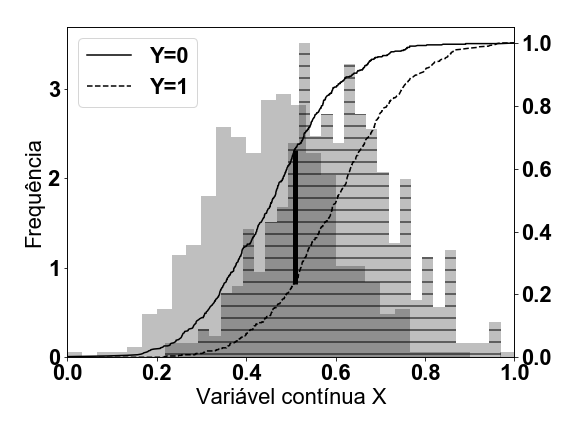
\includegraphics[scale=0.20]{images/KS_teorico.png}
				\label{fig:ksTeorico}
			\end{figure}
			Fonte: \SourcePadrao
		\end{center}
	\end{tcolorbox}


	\begin{tcolorbox}[colback=blue!5!white,colframe=blue!75!black,title=Definição e propriedades,valign=center]\selectFont
	\begin{itemize}
		\item $KS(X,Y) = \operatorname*{arg\_max}_x abs(CDF(x | y=0)- CDF(x | y=1))$
		\item Distância entre as curvas de probabilidades acumuladas.
		\item Mede se a variável binária representa distribuições diferentes.
	\end{itemize}
	\end{tcolorbox}
\end{frame}


\begin{frame}{Modelos de aprendizado de máquina (AM)}

\begin{columns}
	\begin{column}{0.55\textwidth}
		\begin{tcolorbox}[colback=blue!5!white,colframe=blue!75!black,valign=center,title=Regressão logística softmax]\selectFont
			\centering
			\begin{equation} 
			\begin{matrix}
			f_1(X) - \ln Z  & = \ln P(Y=1|X) \\
			\cdots & \cdots \\
			f_c(X) - \ln Z & = \ln P(Y=c|X) \\
			\end{matrix}
			\label{eq:logisticaArray}
			\end{equation}
			
			$\Downarrow$
			
			\begin{equation}
			P(Y=c|X) =softmax(X,c) = \frac{e^{f_c(X)}}{\sum_{k=1}^{K} e^{f_k(X)}}
			\label{eq:softmax}
			\end{equation}
		\end{tcolorbox}
	\end{column}
	\begin{column}{0.45\textwidth}
		\begin{tcolorbox}[colback=blue!5!white,colframe=blue!75!black,valign=center,title=Propriedades]\selectFont
			$\bullet$ Não assume a independência das variáveis.
			
			$\bullet$ Possui saída probabilística.
			
			$\bullet$ As probabilidades reflem o balanceamento das classes.
			
			$\bullet$ Possui saída contínua.
			
			$\bullet$ É um classificador linear.
			
			$\bullet$ É usado em aprendizado profundo.
		\end{tcolorbox}
	\end{column}
\end{columns}

\end{frame}